\newpage
\begin{center}
    \rule{\linewidth}{0.2 mm} \\[0.4 cm]
	{ \huge \bfseries Mini Projects}\\
	\rule{\linewidth}{0.2 mm} \\[1.5 cm]
	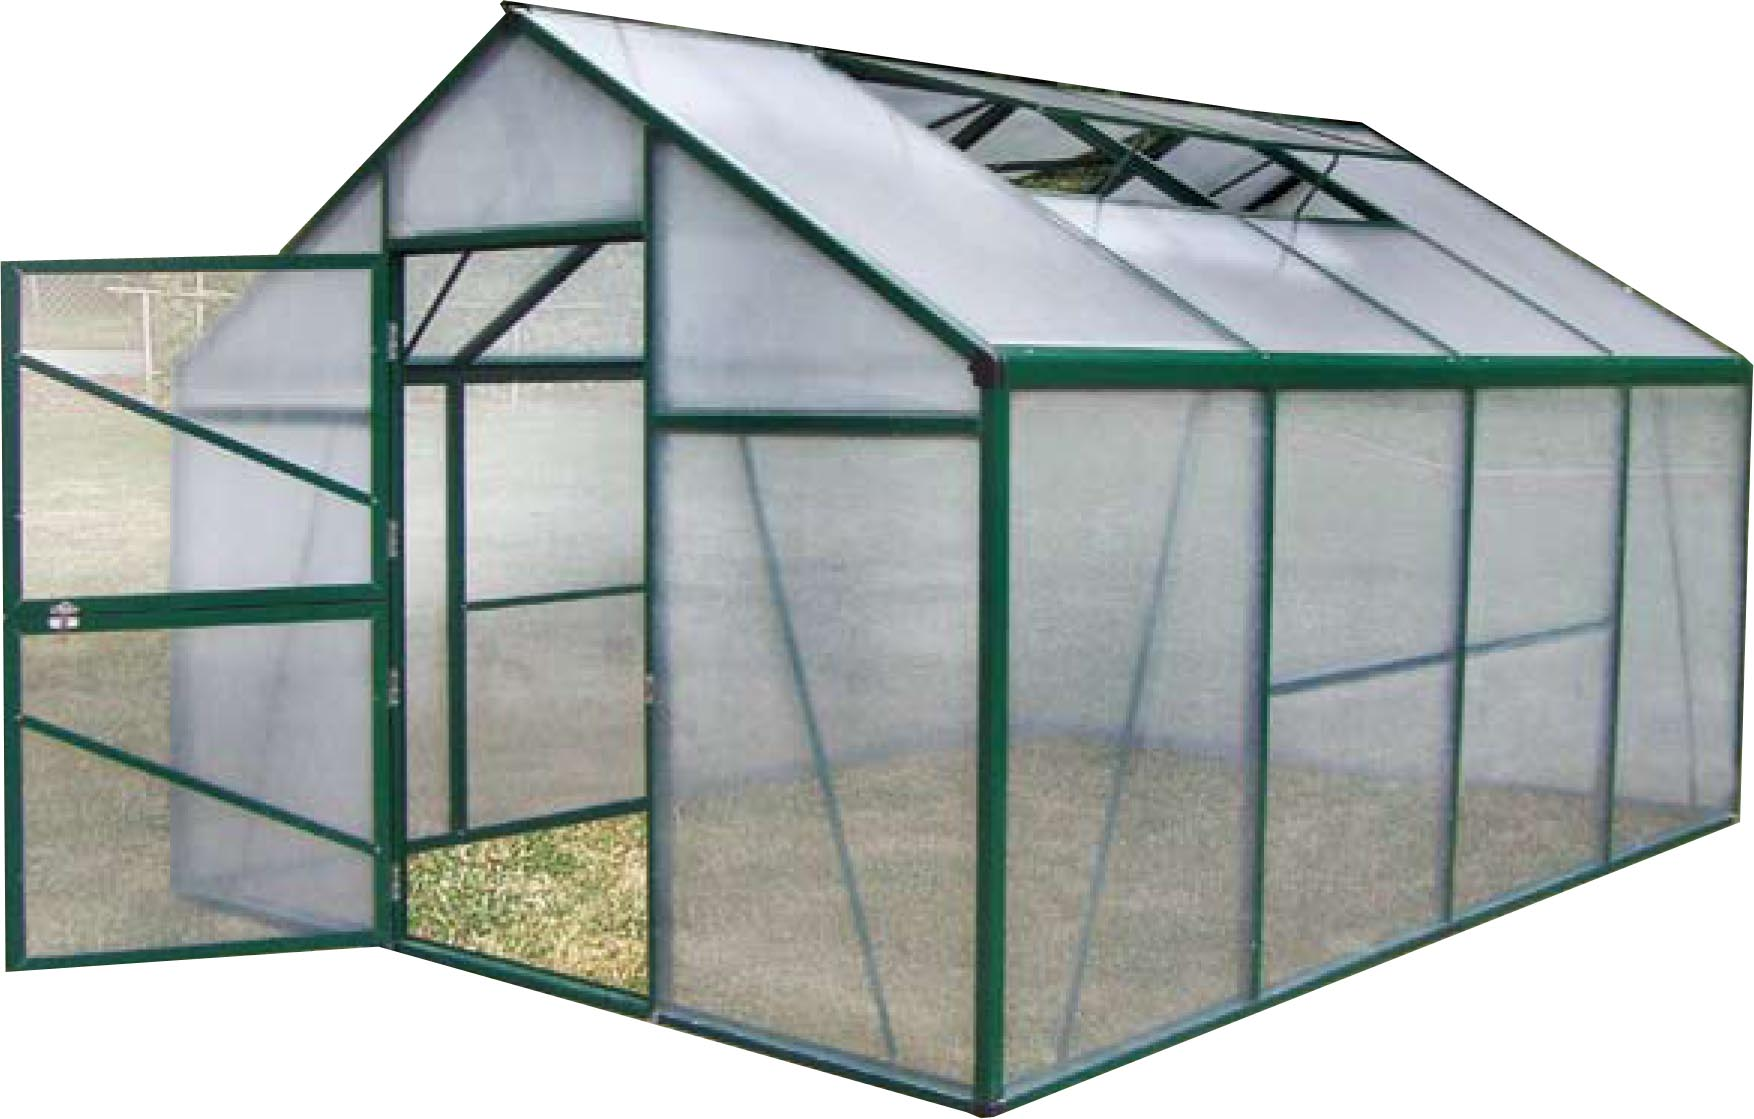
\includegraphics[scale = 0.5]{Figures/Greenhouse.jpg}\\[1 cm]
	\textsc{\Large EEE3096S}\\[0.5 cm]
	\textsc{\large Embedded Systems II}\\[0.5 cm]
	\textsc{\LARGE University of Cape Town}\\[0.5 cm]
\end{center}

\section{Overview}
The mini-project is a chance for you to use what you have learnt in this course and test your problem-solving skills. The projects use everything learnt in the previous practicals - so here's hoping you paid attention and remembered those! All students need to do Mini Project A. Only CS students need to do Mini Project B.

\subsection{Scenario}
A biology student has approached you with the task of monitoring their private greenhouse. They request that you monitor time of day, time since the system has been running, light levels, temperature, and humidity. They have a device that monitors humidity. It outputs an analog voltage between 0 and 3.3V. For testing and development purposes, you decide to use a potentiometer to mimic the humidity sensor. With the experience you've gained working with the Raspberry Pi over the past few months, you decide that this is a good chance to test your newly acquired knowledge and establish an effective development environment for further projects.

The biology student has a computer in their greenhouse that they use to play music to their plants as a part of their research, so they are able to access the Raspberry Pi on location through a terminal or VNC. However, they wish to be able to also monitor the data remotely. They say their younger brother, who plays with Arduinos, has spoken a lot about \href{https://blynk.io/}{Blynk} for IoT devices. You decide to look into these options for remote monitoring. 

The also request that your device output a voltage to their own custom recording equipment. The voltage should be calculated as follows:
$$
V_{out} = \frac{Light Reading}{1023} \times Humidity Voltage Reading
$$
If the output voltage goes under 0.65V or over 2.65V, an alarm should sound. A button should be added to dismiss the alarm, and the alarm should only sound if it the previous alarm dismissal was more than 3 minutes ago (i.e. the alarm can only sound every 3 minutes).\textbf{The three minute timer should start when the alarm is sounded, not when the alarm is dismissed.}


\subsection{Basic Details}
Your objective for Mini Project A and B is to design an environment logger. An environment logger interacts with the world around it by measuring any number of factors from GPS location to air pollution. While a single sensor is useful to monitor a single location, many can be scattered around a broader area to monitor that area as well as any patterns emerging in that broader area.

Project A and B differ in how that data is presented to end users. Project A will require use of a single Raspberry Pi, which relays data to and is controlled via an app on your phone created through Blynk.

Project B requires two Raspberry Pis. Instead of using Blynk, one Pi works as the environment sensor. It will send the gathered data using a protocol called MQTT to a node red server, which will be hosted on the second Raspberry Pi. Users should be able to log in to a hot spot hosted on the second Raspberry Pi and access the Node Red server to see the data being captured.

The objective of these mini-projects is to get some experience on what it might be like to create and deploy a real IoT device - what the pracs in the course have been leading up to!

\section{Mini-Project A}
\label{sec:ProjA}
This project examines ELO5.2, which requires the student to develop a representative embedded system. It requires hardware/software interfacing, so an ADC is sampled by software, and processing operations are applied to read the data. 

\subsection{Pre-Project Requirements}
\begin{itemize}
    \item You will need to have completed all the previous practicals in order to complete this project.
    \item Using the design flows presented in class, we strongly recommend beginning by drawing up an initial design and mapping the required tasks to (at the least) a simple timeline or Gantt chart.
\end{itemize}

\subsection{Outcomes}
In addition to creating a working system, you will learn about the following in this project:
\begin{itemize}
    \item ADC - \href{https://cdn-shop.adafruit.com/datasheets/MCP3008.pdf}{MCP3008}
    \item Temperature sensor - \href{http://ww1.microchip.com/downloads/en/devicedoc/20001942g.pdf}{MCP9700A}
    \item IOT - \href{https://blynk.io/}{Blynk}
\end{itemize}

\subsection{Deliverables}
At the end of this practical, you must:
\begin{itemize}
    \item Demonstrate your working implementation to a tutor through a formal presentation. This will take the form of a formal presentation in a 10 minute slot you will book in advance. See Table \ref{tbl:DemoValidation} for details on the demonstration.
    \item Submit your report to Vula, in the format shown in Table \ref{tbl:flamarks}
    \item For information on the marks and what sections to cover, refer to the marking guide in Section \ref{sec:ProjAMarks}
\end{itemize}

\subsection{Hardware Required}
\begin{tabular}{ll}
\begin{tabular}[c]{@{}l@{}}
\tabitem All hardware from previous pracs\\ 
\tabitem Potentiometer to mimic VPD sensor\\ 
\tabitem LDR\\
\end{tabular} 
&\begin{tabular}[c]{@{}l@{}}
\tabitem ADC\\ 
\tabitem Temperature Sensor\\ 
\\
\end{tabular} 
\end{tabular}

\subsection{System Overview}
Figure \ref{fig:SystemOverview} shows the system overview for the mini project.
\begin{figure}[H]
\centering
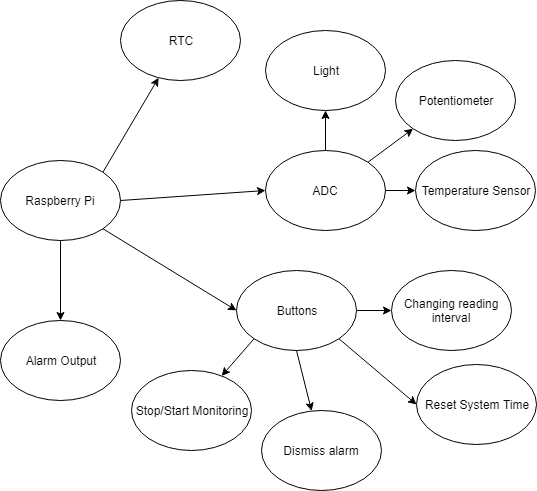
\includegraphics[width=0.8\columnwidth]{Figures/SystemOverview}
\caption{Components of the Mini-Project}
\label{fig:SystemOverview}
\end{figure}

\begin{multicols}{2}
Figure \ref{fig:blynkexample} shows an example of what the app you create in Blynk might look like.
As you can see there's a terminal for accessing the output of the print statements, three values as read from the ADC, and an indicator to indicate if the alarm has gone off. There are various widgets in Blynk. It's suggested you play with your energy budget to develop the most intuitive design and aesthetically pleasing design possible.
\vfill\null
\columnbreak
\begin{figure}[H]
\centering
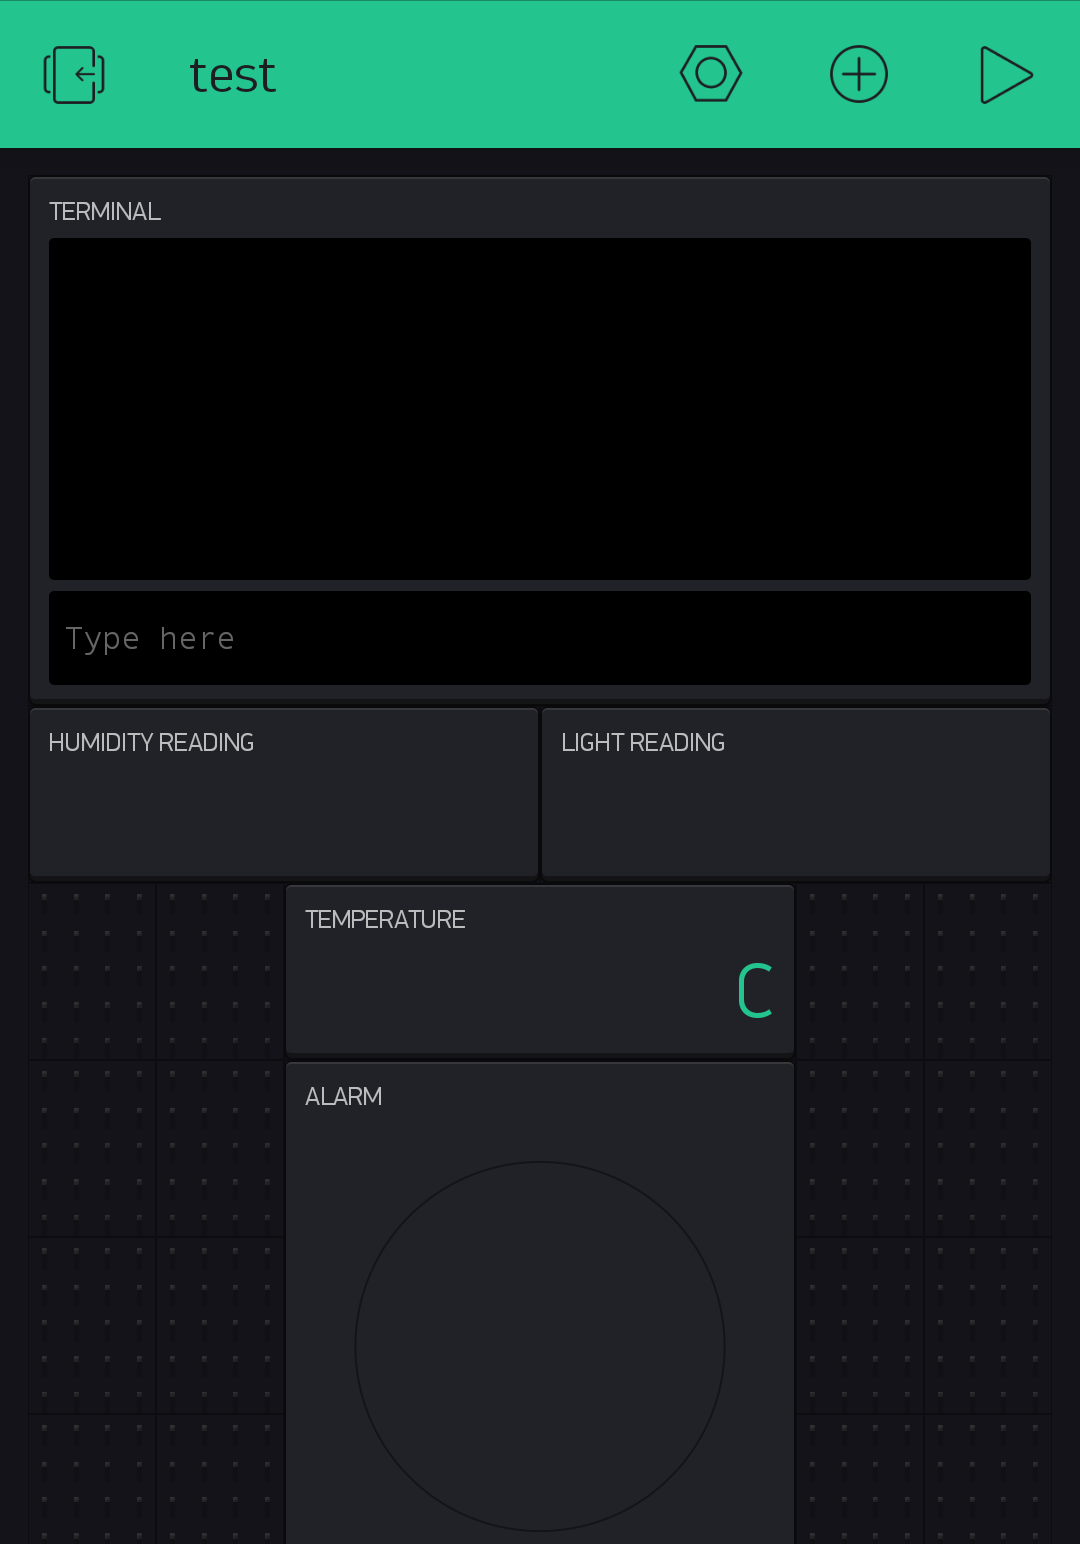
\includegraphics[width=0.75\columnwidth]{Figures/blynkexample}
\caption{Example Blynk Project}
\label{fig:blynkexample}
\end{figure}
\end{multicols}


\subsection{Hardware requirements}
You will need to build your design and demonstrate it to the marker.

\subsection{Software requirements}
You need to do the following:
\begin{itemize}
    \item Set up the RTC. You can use either the Raspberry Pi's supplied kernel driver for an RTC, or you can interface with it as you did in Practical 3.
    \item Create a thread for reading from the ADC. The value read from the temperature sensor needs to be converted to degrees Celsius. See the datasheet (linked above) for the formula.
    \item Create interrupts for all the button functionality (don't forget to debounce your inputs)
    \item Output the correctly calculated voltage over the DAC.
    \item Create an output signal to notify the biology student that there is an issue. You can flash an LED using a PWM signal, you can play audio through the audio jack, or you can buy a buzzer from WhiteLab. 
    \item In the main() loop, print values to the screen as described in Section \ref{sec:ProjDescription}
\end{itemize}

\subsection{Description}
\label{sec:ProjDescription}
\begin{itemize}
    \item The system should have hard-coded thresholds. When a value read by the device goes over a threshold, an alarm should sound. A button must be pressed to dismiss the alarm.
    \item By default, the system continuously monitors the sensors every 1s using this format:
    \begin{table}[H]
    \centering
    \begin{tabular}{|l|l|l|l|l|l|l|}
    \hline
    RTC Time & Sys Timer & Humidity  & Temp  & Light & DAC out & Alarm \\ \hline
    10:17:15 & 00:00:00 & 0.5 V &   25 C    & 595 & 0.29V&* \\ \hline
    10:17:20 & 00:00:05 & 1.5 V &   25 C    & 595 & 0.87V&* \\ \hline
    10:17:25 & 00:00:10 & 1.7 V &   25 C    & 595 & 0.98V&  \\ \hline
    10:17:30 & 00:00:15 & 2.2 V &   25 C    & 782 & 1.68V&  \\ \hline
    10:17:35 & 00:00:20 & 3.3 V &   25 C    & 998 & 3.22V&  \\ \hline
    \end{tabular}
    \end{table}
    Notice how the alarm flag is still active at 10:17:20, as it is only dismissed before the reading at 10:17:25. Also note that even though the DAC out value exceeds the alarm threshold at time 10:17:35, no alarm is sounded as the last alarm was sounded less than three minutes prior. 
    \item The reset switch resets the system timer and cleans the console
    \item The frequency switch changes the frequency of the monitoring. The possible frequencies are 1s, 2s and 5s. The frequency must loop between those values per event occurrence.
    \item The stop switch stops or starts the monitoring of the sensors. The system timer is not affected by this functionality.
    \item Blynk must be used to:
    \begin{itemize}
        \item View live logging information (System time and ADC values)
        \item Be notified of alarms
    \end{itemize}
\end{itemize}

\subsection{Marking Guide}
\label{sec:ProjAMarks}
\begin{longtable}[c]{|l|l|l|}
\caption{Project A marking Guide}
\label{tbl:flamarks}\\
\hline
\textbf{Heading} & \textbf{Report} & \textbf{Demo} \\ \hline
\endfirsthead
%
\endhead
%
Introduction & \begin{tabular}[c]{@{}l@{}}Provide a short introduction ($\sim \frac{1}{2}$ page)\\ to your project explaining your main\\ design choices and how the report has\\ been structured (15 marks)\end{tabular} & \begin{tabular}[c]{@{}l@{}}Introduce yourselves and\\ your project. {[}8 marks{]}\end{tabular} \\ \hline
Requirements & \begin{tabular}[c]{@{}l@{}}The requirements section should\\ provide a refined UML Use Case\\ diagram of the system, according to\\ your implementation, and any\\ accompanying text that is needed to\\ clarify the requirements.\\ Highlight any departures or additions\\ that you may have made compared to\\ the original project description given in\\ this document. {[}15 marks{]}\end{tabular} & \begin{tabular}[c]{@{}l@{}}Have an (at least draft)\\ UML Use Case to show\\ the tutor. Show this\\ briefly, indicating any\\ departures/additions.\\ {[}6 marks{]}\end{tabular} \\ \hline
\begin{tabular}[c]{@{}l@{}}Specification \\ and Design\end{tabular} & \begin{tabular}[c]{@{}l@{}}This section should provide a UML\\ State Chart describing the main\\ operation. Add a UML class or\\ deployment diagram (or other suitable\\ diagram) to indicate the structuring of\\ your implementation (e.g. code\\ modules/classes you may be using).\\ You don’t need to provide fine detail of\\ the system, the diagram(s) can be e.g.\\ at the level of functions. You should\\also include a circuit diagram {[}20 marks{]}\end{tabular} & \begin{tabular}[c]{@{}l@{}}Briefly show your design,\\ you need not show more\\ than one rough diagram\\ (e.g. draft state chart) to\\ the tutor. {[}10 marks{]}\end{tabular} \\ \hline
Implementation & \begin{tabular}[c]{@{}l@{}}This section should give some snippets\\ of important code and explanations for\\ this (or referring to particular\\ functions in code files). The point here\\ is elaborating any parts of the State\\ Chart that are not so straightforward\\ to turn into code. {[}20 marks{]}\end{tabular} & \begin{tabular}[c]{@{}l@{}}You should have a code\\ file open already (e.g.\\ where the main function\\ is) before you start the\\ demo. Briefly confirm to\\ the tutor that this is part\\ of the program that will be\\ demoed. {[}6 marks{]}\end{tabular} \\ \hline
\begin{tabular}[c]{@{}l@{}}Validation and\\ Performance\end{tabular} & \begin{tabular}[c]{@{}l@{}}Provide at least a paragraph or two\\ explaining the performance of the\\ system. A snapshot could be included\\ and you could show test cases where\\ you have tested that the system works\\ reliably (e.g. using a powersupply to set \\ the value given to the ADC). {[}20\\ marks{]}\end{tabular} & \begin{tabular}[c]{@{}l@{}}This is a main aspect of\\ the demonstration.\\ See Validation Check\\ Sheet in Section \ref{sec:ProjAValidation}.\\ {[}40 marks{]}\end{tabular} \\ \hline
Conclusion & \begin{tabular}[c]{@{}l@{}}Give a summary of the extent that the\\ system was found to be successful.\\ Discuss if you think that a system\\ working in this way might be\\ considered a potentially useful product.\\ {[}10 marks\end{tabular} & \begin{tabular}[c]{@{}l@{}}End you demo with a\\ short conclusion, reflect\\ on the activity. {[}10 marks{]}\end{tabular} \\ \hline
References & Provide a few references if relevant. & Questions {[}20 marks{]} \\ \hline
Total & 100 &  \\ \hline
\end{longtable}

\subsection{Project A Validation Sheet}
\label{sec:ProjAValidation}
\begin{table}[H]
\centering
\resizebox{\textwidth}{!}{%
\begin{tabular}{|l|l|l|r|c|c|c|}
\hline
\multicolumn{3}{|l|}{{\ul \textbf{Project Validation Sheet}}}  & \multicolumn{4}{l|}{\begin{tabular}[c]{@{}l@{}}\textbf{Marked by:} \\ \\\end{tabular}} \\ \hline
\multicolumn{7}{|l|}{\begin{tabular}[c]{@{}l@{}}\textbf{Student Numbers:} \\ \\ \\\end{tabular}} \\ \hline
\textbf{Category} & \textbf{Item} & \textbf{Description} & \multicolumn{1}{c|}{Max Mark} & \begin{tabular}[c]{@{}c@{}}Attempt\\ 1\end{tabular} & \begin{tabular}[c]{@{}c@{}}Attempt\\ 2\end{tabular} & \begin{tabular}[c]{@{}c@{}}Attempt\\ 3\end{tabular} \\ \hline
 &  &  &  \textbf{Date:} & \begin{tabular}[c]{@{}l@{}} \\ \\\end{tabular} &  & \\ \hline
\textbf{Blynk} & \begin{tabular}[c]{@{}l@{}}Connected \\ and responds\end{tabular} & \begin{tabular}[c]{@{}l@{}}Blynk should connect to\\ the pi (2) and respond to \\ changes on the pi (5 - ldr, \\ pot, temp, alarm, start/stop \\ log)\end{tabular} & 7 &  &  &  \\ \hline
\textbf{} & Design & \begin{tabular}[c]{@{}l@{}}All features of the should\\ be reflected in the widgets\\ used in Blynk\end{tabular} & 5 &  &  &  \\ \hline
 &  & \begin{tabular}[c]{@{}l@{}}The use of widgets should\\ be aesthetically pleasing as\\ well as intuitive (use of labels,\\ placement of widgets)\end{tabular} & 2 &  &  &  \\ \hline
ADC & Temperature & \begin{tabular}[c]{@{}l@{}}Temperature reported on is\\ accurate and responds to \\ input (warming up when \\ sensor is held, etc)\end{tabular} & 2 &  &  &  \\ \hline
 & Potentiometer & \begin{tabular}[c]{@{}l@{}}Responds to changes input, \\ reading displayed is between\\ 0 and 3.3V\end{tabular} & 2 &  &  &  \\ \hline
 & Light sensor & Voltage divider & 2 & \begin{tabular}[c]{@{}l@{}} \\ \\\end{tabular} &  &  \\ \hline
 &  & \begin{tabular}[c]{@{}l@{}}Reports a value between\\ 0 and 1023\end{tabular} & 2 &  &  &  \\ \hline
\begin{tabular}[c]{@{}l@{}}Buttons/\\ Logging\end{tabular} & Implementation & \begin{tabular}[c]{@{}l@{}}Uses interrupts (1 ea) and \\ debouncing (1 ea)\end{tabular} & 8 &  &  &  \\ \hline
 & Interval Reading & Changes between 1, 2 and 5s & 3 & \begin{tabular}[c]{@{}l@{}} \\ \\\end{tabular} &  &  \\ \hline
 & Reset SysTime & Resets system time to 0 & 1 & \begin{tabular}[c]{@{}l@{}} \\ \\\end{tabular} &  &  \\ \hline
 & Dismiss Alarm & \begin{tabular}[c]{@{}l@{}}Clears alarm and outputs \\ message saying so.\end{tabular} & 2 &  &  &  \\ \hline
 & \begin{tabular}[c]{@{}l@{}}Stop/Start \\ logging\end{tabular} & \begin{tabular}[c]{@{}l@{}}Pauses the print out to \\ system console, but timer \\ continues increasing\end{tabular} & 1 &  &  &  \\ \hline
Alarm & Implementation & Calculation implemented & 1 & \begin{tabular}[c]{@{}l@{}} \\ \\\end{tabular} &  &  \\ \hline
 &  & Outputs correct voltage & 1 & \begin{tabular}[c]{@{}l@{}} \\ \\\end{tabular}  &  &  \\ \hline
 &  & \begin{tabular}[c]{@{}l@{}}Can't sound more often \\ than 3 minute intervals\end{tabular} & 1 &  &  &  \\ \hline
Mark &  &  & 40 & \begin{tabular}[c]{@{}l@{}} \\ \\\end{tabular} &  &  \\ \hline
\end{tabular}%
}
\end{table}
\section{Mini-Project B}
This project is for CS students only. Of course, if you'd like to attempt, you can.\\

\subsection{Scenario}
The biology student appreciates the work you have done developing a rough prototype. Their research has started gaining ground, and more people are becoming interested in their research. Because you did such a good job of developing the base system, the biology student has asked you to develop a means of a system where anyone can access their data. Being competent developers, well aware of web development, as well as being aware of the world of embedded systems you decide to use MQTT to transfer data. You want to make the system as accessible as possible, so you decide to use a low-cost Raspberry Pi to host a Node-Red server. For the sake of the prototype, you create a hotspot on the Raspberry Pi that people can connect to in order to access the server. You decide on the following design, as shown in Figure \ref{fig:NodeRed}:

\begin{figure}[H]
\centering
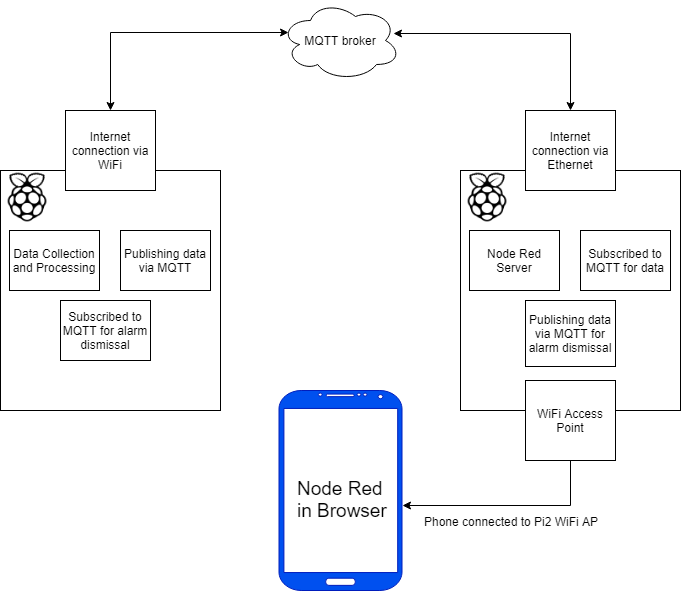
\includegraphics[width=1\columnwidth]{Figures/NodeRed}
\caption{Project B System Overview}
\label{fig:NodeRed}
\end{figure}

\subsubsection{Overview}
For this task, two Raspberry Pis are required. Both are required to publish and subscribe to data. One Pi must publish the recorded data, and subscribe to an alarm dismissal signal. A second Pi should publish an alarm dismissal message and subscribe to the data collected by the first Pi. A web page must be hosted on the second Pi, and it's WiFi interface should be turned into an access point. Devices should be able to connect to this access point, and view a web page which can mimic the Blynk App designed in Mini-Project A. For the MQTT broker, you can use a \href{https://diyprojects.io/8-online-mqtt-brokers-iot-connected-objects-cloud/}{publicly available one}, or host one on one of the Pis.

Essentially, this is a repeat of the first project, but using a second Raspberry Pi with MQTT and Node Red as opposed to Blynk.

\subsubsection{Outcomes}
You will learn about:
\begin{itemize}
    \item MQTT (It's suggested you read \href{https://randomnerdtutorials.com/what-is-mqtt-and-how-it-works/}{this introduction to MQTT} and \href{https://cookbook.nodered.org/mqtt/}{MQTT on NodeRed}
    \item NodeRed (It's suggested you read \href{https://nodered.org/docs/getting-started/raspberrypi}{Getting Started with NodeRed on the RaspberryPi} to get started. There's also a nice plugin for good looking dashboards \href{https://flows.nodered.org/node/node-red-dashboard}{here}. You can also read the \href{https://learn.adafruit.com/raspberry-pi-hosting-node-red}{Adafruit Guide}.)
    \item Hosting an access point on the Pi. Notes are available in the lab handbook. 
\end{itemize}

\subsubsection{Deliverables}
At the end of this practical, you must
\begin{itemize}
    \item Demonstrate your implementation to a tutor. They will log in to your hotspot through their phone, view values, and adjust the alarm threshold.
    \item Submit a short write up. See the marking guide in section \ref{sec:ProjBMarks}
\end{itemize}

\subsubsection{Hardware Required}
You require the hardware from Project A, as well as a secondary Pi.

\subsubsection{Software Requirements}
\begin{itemize}
    \item You need to use an MQTT broker to publish and subscribe to messages relating to your practical. 
    \item You need to create a Node Red server that displays your data gathered from the first Raspberry Pi. 
    \item You will also need to have an option to adjust the alarm threshold from the NodeRed server.
\end{itemize}

\subsubsection{Marking Guide}
\label{sec:ProjBMarks}
\begin{table}[H]
\centering
\caption{The Write Up Format For mini-project B}
\label{tbl:ProjBMarks}
\begin{tabular}{|l|l|l|}
\hline
\textbf{Section of Report} & \textbf{Description} & \textbf{Marks} \\ \hline
\textbf{Introduction} & An introduction to what's new in this project & 10 \\ \hline
\textbf{Design} & \begin{tabular}[c]{@{}l@{}}Design of the system. Design of the server. \\ Talk about the stack used for development. \\ Include UML and block diagrams, and \\ mention any hardware/software\\ interfacing issues.\end{tabular} & 30 \\ \hline
\textbf{\begin{tabular}[c]{@{}l@{}}Implementation/\\ Build Proces\end{tabular}} & \begin{tabular}[c]{@{}l@{}}Some code snippets and steps in building \\ the device and server.Can think of this as a\\ simple methodology.\end{tabular} & 15 \\ \hline
\textbf{Instructions for use} & \begin{tabular}[c]{@{}l@{}}How to operate the system. You should \\ include some screenshots and photos.\end{tabular} & 15 \\ \hline
\textbf{Testing/Results} & \begin{tabular}[c]{@{}l@{}}How did you ensure your system works? \\ What did you do to test the functionality, \\ and what were the results? You can include\\ screenshots or photos, but you need to talk \\ about them (it's not enough to just have a \\ photo).\end{tabular} & 20 \\ \hline
\textbf{Conclusions} & \begin{tabular}[c]{@{}l@{}}How well did your system work? Did you \\ achieve the objectives? What could you do \\ to improve the system?\end{tabular} & 10 \\ \hline
\textbf{TOTAL} &  & \textbf{100} \\ \hline
\end{tabular}%
\end{table}

\subsubsection{Project B Validation Guide}
\label{sec:ProjBValidation}
\begin{table}[H]
\centering
\caption{Project B Demo Marks}
\label{tbl:ProjBValidation}
\resizebox{\textwidth}{!}{%
\begin{tabular}{|l|l|l|l|l|}
\hline
\multicolumn{2}{|l|}{\textbf{ProjB Validation Sheet}} & \multicolumn{3}{l|}{Marked By:} \\ \hline
\multicolumn{5}{|l|}{Student Numbers:} \\ \hline
\textbf{Component} & \textbf{Category} & \textbf{Description} & \textbf{Max marks} & \textbf{Mark} \\ \hline
\textbf{Hotspot} & Connectivity & \begin{tabular}[c]{@{}l@{}}Viewable in WiFi Menu \\ from phone\end{tabular} & 1 &  \\ \hline
 &  & Tutor can connect to it & 1 &  \\ \hline
\textbf{Node Red} & Implementation & WebPage is accessible & 1 &  \\ \hline
 &  & Starts on Boot & 1 &  \\ \hline
 & Design & \begin{tabular}[c]{@{}l@{}}All features of the\\ EnviroLogger should be\\ reflected in the webpage\\  (5 - LDR, pot, temp, \\ alarm, start/stop log)\end{tabular} & 5 &  \\ \hline
 &  & \begin{tabular}[c]{@{}l@{}}The use of widgets should \\ be aesthetically pleasing as \\ well as intuitive (use of labels, \\ placement of components)\end{tabular} & 3 &  \\ \hline
 &  & \begin{tabular}[c]{@{}l@{}}Can adjust the alarm \\ threshold (1) and is tested (2)\end{tabular} & 3 &  \\ \hline
 \textbf{Questions} & & & 5 &\\ \hline
\textbf{Marks Obtained} &  &  & \textbf{20} &  \\ \hline
\end{tabular}%
}
\end{table}




